\chapter{A Unified Model for Multi-Modal Attention} 
\label{chapter-unified} 

The purpose of using EMMA is to help the multi-modal network (MMN) to handle failing modes, and more generally, to figure out the relative emphases to be placed on the different modalities depending on their general contributions. The literature review\footnote{Chapter \ref{chapter-literature-review}} discussed self-attention and crossmodal attention mechanisms, used to highlight information inside a specific mode, such as certain regions in an image or a set of frequencies in a sound. The difference between these two mechanisms is that self-attention only relies on information from the mode itself as a context, whereas crossmodal attention uses information from all the available modes. In combination with EMMA, we claim to have all the ingredients to construct a complete multi-modal network like humans. As a reminder, human's multi-modal attention consists of three different components: exogenous, endogenous and crossmodal attention. Attention is endogenous when we voluntary choose to attend to something whereas exogenous attention is triggered by the sudden onset of an unexpected event \citep{crossmodal}. One way of constructing an endogenous module would be as a block of $M$ self-attentions, where each self-attention is dedicated to one specific mode. On the other hand, the attention module developed in this work can be considered as an equivalence to exogenous attention used by humans to robustly handle abnormal situations.

\begin{figure}[hbt!]
\centering
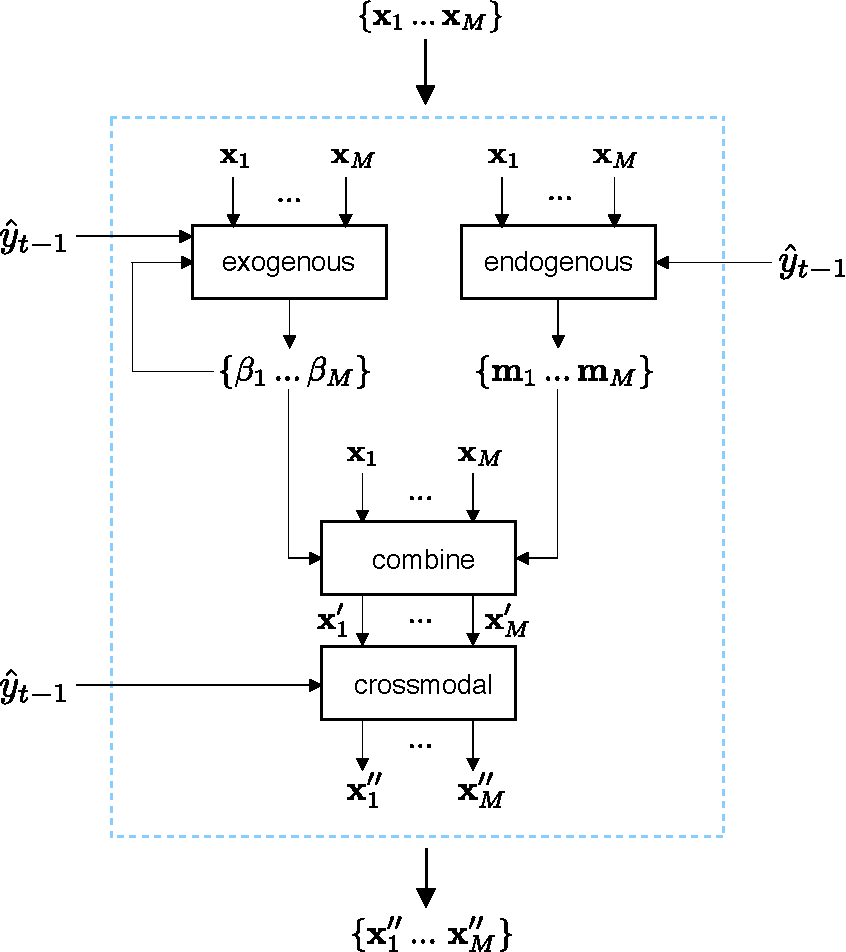
\includegraphics[scale=0.75]{figures/unified}
\caption{A possible architecture for a unified multi-modal attention}
\label{fig:complete-model}
\end{figure}

With this in mind, we present a unified model (see Figure \ref{fig:complete-model}) combining all the strengths of each type of attention. First, the attention masks $\beta_i$ computed by the exogenous model, and the attention masks $\mathbf{m}_i$ computed by the endogenous module, are combined to obtain the resulting masks $\beta_i\mathbf{m}_i$. These mask will highlight the most important modes, and on an intra-modal level attend to the most relevant regions. The masks $\beta_i\mathbf{m}_i$ are then applied to the input sample, which is passed through the crossmodal module. Finally, the processed input $\{\mathbf{x}''_1\,...\,\mathbf{x}''_M\}$ is forwarded to the MMN. In addition, the complete module can further be refined by inserting feedback loops from the previously predicted output to the separate modules, as it is often done in the literature \citep{afouras, attention-need, bahdanau}. For example, in a self-driving system, the attention module could improve its focus to different regions of the input image depending on the previously detected cars. It is worth mentioning that the proposed architecture is only a generalization of current attention modules such as in \citep{afouras}, supplemented with an exogenous component.


